% Pascal: hexagon ABCDEF inscribed in an ellipse; X = AB.DE, Y = BC.EF, Z = CD.FA lie on the Pascal line.
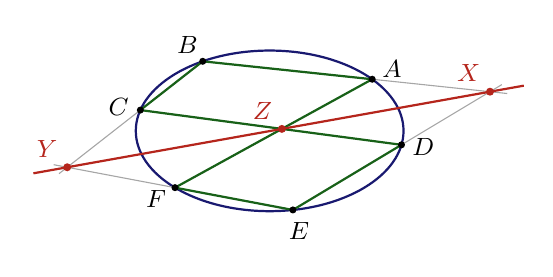
\begin{tikzpicture}[scale=0.85,font=\small]
\draw[MidnightBlue,thick] (0,0) ellipse (2.0000 and 1.2000);
\draw[black!35] (-1.0000,1.0392) -- (3.5497,0.5579);
\draw[black!35] (0.3473,-1.1818) -- (3.4688,0.6912);
\draw[black!35] (-1.0000,1.0392) -- (-3.1461,-0.6389);
\draw[black!35] (0.3473,-1.1818) -- (-3.2269,-0.5056);
\draw[black!35] (-1.9319,0.3106) -- (0.3094,0.0125);
\draw[black!35] (-1.4142,-0.8485) -- (0.2783,0.0820);
\draw[ForestGreen!70!black,thick] (1.5321,0.7713) -- (-1.0000,1.0392);
\draw[ForestGreen!70!black,thick] (-1.0000,1.0392) -- (-1.9319,0.3106);
\draw[ForestGreen!70!black,thick] (-1.9319,0.3106) -- (1.9696,-0.2084);
\draw[ForestGreen!70!black,thick] (1.9696,-0.2084) -- (0.3473,-1.1818);
\draw[ForestGreen!70!black,thick] (0.3473,-1.1818) -- (-1.4142,-0.8485);
\draw[ForestGreen!70!black,thick] (-1.4142,-0.8485) -- (1.5321,0.7713);
\draw[BrickRed,thick] (-3.5299,-0.6342) -- (3.7975,0.6755);
\fill (1.5321,0.7713) circle (1.5pt) node[shift={(0.250,0.126)}] {$A$};
\fill (-1.0000,1.0392) circle (1.5pt) node[shift={(-0.194,0.202)}] {$B$};
\fill (-1.9319,0.3106) circle (1.5pt) node[shift={(-0.276,0.044)}] {$C$};
\fill (1.9696,-0.2084) circle (1.5pt) node[shift={(0.278,-0.029)}] {$D$};
\fill (0.3473,-1.1818) circle (1.5pt) node[shift={(0.079,-0.269)}] {$E$};
\fill (-1.4142,-0.8485) circle (1.5pt) node[shift={(-0.240,-0.144)}] {$F$};
\fill[BrickRed] (3.2921,0.5851) circle (1.7pt) node[above left,BrickRed] {$X$};
\fill[BrickRed] (-3.0246,-0.5439) circle (1.7pt) node[above left,BrickRed] {$Y$};
\fill[BrickRed] (0.1825,0.0293) circle (1.7pt) node[above left,BrickRed] {$Z$};
\end{tikzpicture}
